\section{Connecting to WIFI}
To be able to connect to a wifi you're going to add a wifi connection manually in the phone. 

\subsection{Do Once: download and install}\label{subsec:wifi_once}
\begin{enumerate}
    \item "wifi analyzer" \url{http://apkfind.com/dl5/apk/2018/4/8/com.farproc.wifi.analyzer_139.apk?id=com.farproc.wifi.analyzer&f=Wifi%20Analyzer_3.11.2_apk-dl.com.apk}. 
    
    \item "Wifi connecter Library" \url{http://apkfind.com/dl5/apk/2016/11/8/com.farproc.wifi.connecter_16.apk?id=com.farproc.wifi.connecter&f=Wifi%20Connecter%20Library_2.0.3_apk-dl.com.apk}
    \item Install QuickEdit from \url{https://apk-dl.com/quickedit-text-editor-writer-code-editor/com.rhmsoft.edit}
    \item Install the "Edit wifi settings" "app" I created, OR:
    \item you can create it yourself with tasker by importing the task xml code listed in \cref{app:E} and exporting the task as APK. (this way you can open the wifi settings after tasker and your file explorer have been locked by the productivity lock).
    \begin{enumerate}
        \item For Tasker V5.2.bf1 You are required to get the exact same tasker factory version as you have the Tasker app version. The steps required to create the task and consequently the app, were: 
        \item Create a new task in Tasker. 
        \item Press the "+" symbol. 
        \item Click "Code". 
        \item Select "Run Shell" 
        \item At command, enter:
\begin{verbatim}
am start -a android.intent.action.VIEW -c android.intent.category.DEFAULT -d "file:///data/misc/wifi/wpa_supplicant.conf" -t "text/plain"    
\end{verbatim}        
        \item Leave Timeout(Seconds) at 0 
        \item Mark the checkbox at: "Use Root" 
        \item Leave the rest blank/unchanged. 
        \item Hit the back arrow. 
        \item Now you can run the task by pressing the "play" button in the bottom left.
        \item To export the task as an app first install taskbuilder from \url{https://apkpure.com/tasker-app-factory/net.dinglisch.android.appfactory/download?from=details}
        \item Select an icon for the task (9 bloks bottom middle of screen.)
        \item Long press task>export>as app.
        \item The file was only openable by the QuickEdit app. The others did not get access.
    \end{enumerate}
    \begin{figure}[H]
        \centering
        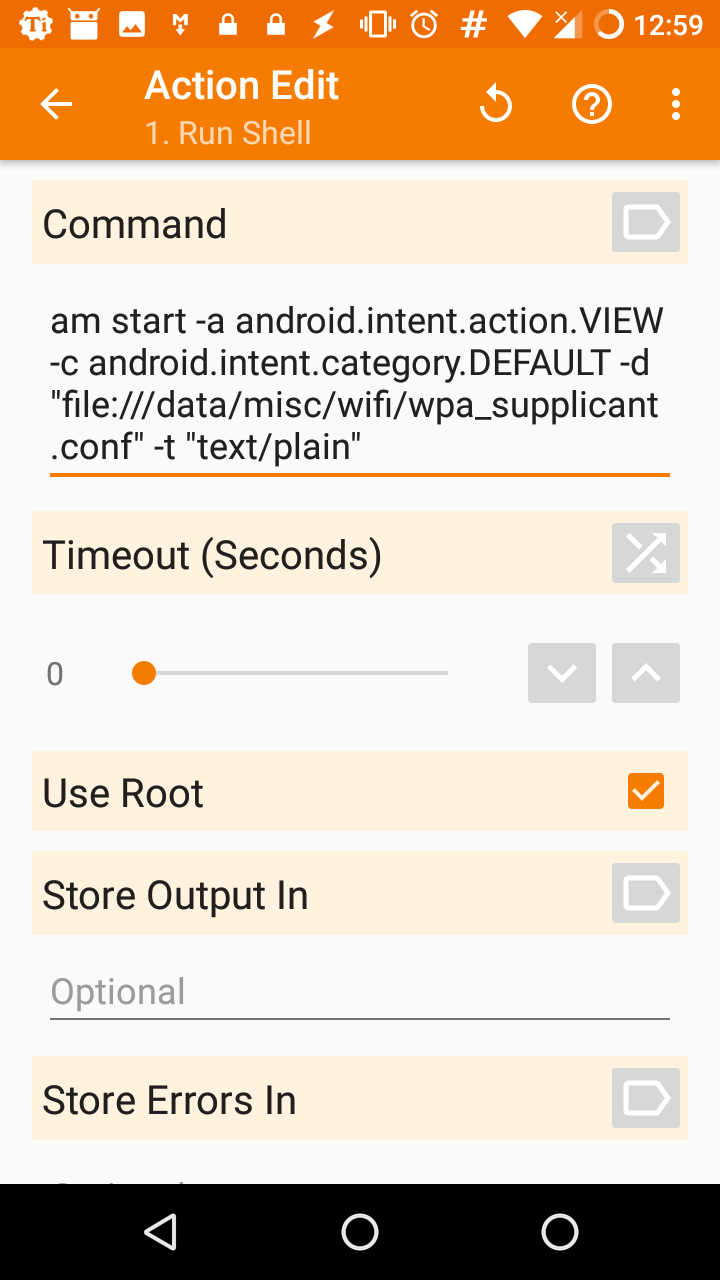
\includegraphics[width=10cm,height=10cm,keepaspectratio]{images/tasker.png}
        \caption{Example of the input in the task at tasker}
        \label{fig:my_label}
    \end{figure}
    
\end{enumerate}

\subsection{Do everytime you connect to a NEW, UNKOWN wifi network}
\begin{enumerate}
    \item Find the BSSID using the app "wifi analyzer" and copy it.
    \item Open the "OpenWifiSettings" app (from cloud, or created with Tasker or restored from Titanium backup) (this opens the wifi configuration file in app "QuickEdit".
    \item Now you want to create the network settings directly in the file where android normally stores it if you add a new wifi network through network settings. To make it easier you can:
    \item OPTION I: Use the template given in \cref{app:D}, by copying an example network of that text. 
    \item OPTION II: OR you can let the app "full wifi" create a new template for that network for you. Either way you still need to know what the netwerk settings must be. In "full wifi:" \textgreater Click: add new network\textgreater select required settings\textgreater 
    \item Next, open the app "OpenWifiSettings".
            \begin{itemize}
            \item OPTION I: If it exists remove the network settings for that BSSID. Then add the text of the network you copied from \cref{app:D} and modify the settings/text (e.g. BSSID, password, username, authentication method etc) to what they need to be for your new network.)
            \item OPTION II: Find the BSSID and edit the settings to what they should be, if you  
            \item Save the file by long pressing the pencil symbol in the top right of QuickEdit.
        \end{itemize}

    \item Turn wifi on and of to re-initialize the modified //data/misc/wifi/wpa\_supplicant.conf file.
    \item After storing the connection settings for a specific wifi network, you can connect to it in (at least) 2 ways:
    \begin{itemize}
        \item You can connect by clicking the wifi network name(ssid) in the dragdown screen/widget from the normal android homescreen. But that might bring you to wifi settings (which are locked with applock) and ask for a password the first time, click backbackback till you're in the homescreen again without entering any pathword. It will now connect to the ssid you've chosen, or else retry. 
        \item Or you can open the app "wifi analyzer" and long press the wifi network ssid, press connect. It should then automatically connect to the wifi. If you cannot press connect without entering a password, you did not enter the correct data in the wpa\_supplicant.conf file. Please retry.
        
    \end{itemize}
    \item Todo: Create a tasker apk replaces the normal wifi settings interface of android. By asking the user for the input using a dropdownbox listing connection type options and password etc, to prevent typos in the .conf file. 
\end{enumerate}

\section{Summary Tasker}
Tasker is used for the following applications. (how it is used in tasker){what the filetype is stored as}:
\begin{enumerate}
    \item Copying the whatsapp media (as task and profile at 3:42-5:00) {Cloud:xml,.prf.xml}
    \item Copying the camera images (as task and profile at 3:00-3:40){Cloud:xml,.prf.xml}
    \item App to open wifisettings (task named OpenWifiSettings3){Cloud:xml,apk}
    \item app to reset Davdroid (task named ResetDAVdroid){Cloud:xml,apk}
    \item app to reset Taskwarrior (task named ResetTaskwarrior){Cloud:xml,apk}
\end{enumerate}

\section{Downloading data from phone:}
Open location of sdcard with: 
\begin{verbatim}
adb shell cd $EXTERNAL_STORAGE    
\end{verbatim}
List files in Sdcard with:
\begin{verbatim}
adb shell ls $EXTERNAL_STORAGE    
\end{verbatim}
Copy file from External SD card:
\begin{enumerate}
    \item adb root
    \item adb shell cd root
    \item adb shell df
    \item Inspect those values to get the path of the external sd card. For me it was:
\begin{verbatim}
/mnt/media_rw/17EE-2356
\end{verbatim}
    \item copy the file to the location of your "py\_cmd.exe" with:
\begin{verbatim}
adb pull /mnt/media_rw/17EE-2356/contacts.vcf
\end{verbatim}
\end{enumerate}

\section{Softbricked your phone again with incorrect wifi edit}
\subsection{Scenario}
If you copy paste a wifi from the text editor and don't add the correct code at the bottom, you softbrick your phone. To fix it:

\subsection{If you need immediate reboot, losing wifi settings}
\begin{enumerate}
    \item hold power+volume down.
     \item recovery mode
    \item advanced
    \item file manager,
    \item browse to
    \item \verb+/data/misc/wifi/wpa_supplicant.conf+
    \item rename the file to
    \item \verb+adb pull /data/misc/wifi/wpo_supplicant.conf+
    
    \item now you can reboot safely but lost your wifi. To fix your wifi settings again (by removing the invalid one).
\end{enumerate}


\subsection{Unbrick and keep wifi settings}
\begin{enumerate}
    \item open \verb+py_cmd.exe+ in for example \verb+c:/path with space/py_cmd.exe+
    \item adb devices
    \item (wpa if you did not change the name)
    \item \verb+adb pull /data/misc/wifi/wpo_supplicant.conf+
    \item Delete messed up entry from conf file with notepad.
    \item rename file to \verb+wpa_supplicant.conf+
    \item \verb+adb push "c:/path with space/wpa_supplicant.conf" /data/misc/wifi/wpa_supplicant.conf+

    \item for me: 
\begin{comment}
adb root

adb push "E:/18-09-19 Document structure/personal/Automation and Systems/Android/2018-09-22 transfer and adb/Minimal ADB and Fastboot_techbeasts/wpa_supplicant.conf" ///data/misc/wifi/wpa_supplicant.conf
\end{comment}
\end{enumerate}

\subsection{lesson}
To add a new wifi network:
\begin{enumerate}
    \item open the app wifi analyzer, 
    \item and press the wifi network you want to add, 
    \item then enter a password
    \item store the network
    \item Then open self "created" (tasker) app open wifi settings and change the password.
    \item \textbf{DO NOT COPY PASTE AN EXISTING WIFI NETWORK TO MODIFY IT,THAT WILL SOFTBRICK YOUR PHONE}
\end{enumerate}